\chapter{Mezuro: Uma plataforma de Monitoramento de Código Fonte}

%Introdução
A prática da engenharia de software exige compreensão do sistema desenvolvido como um todo, onde o código-fonte é uma das partes mais importantes. O engenheiro de software precisa analizar um código-fonte diversas vezes, seja para desenvolver novas funcionalidades ou melhorar as existentes \cite{meirelles2010mezuro}.
%
Como parte fundamental do projeto de software, o código-fonte é um dos principais artefatos para avaliar sua qualidade \cite{meirelles2009crab}. Essas avaliações não são meramente subjetivas, sendo necessário extrair informações que possam ser replicadas e entendidas da mesma forma, independente de quem analisa o código. As métricas de código-fonte permitem esse tipo de avaliação pois possibilitam analisar, de forma objetiva, as principais características para aceitação de um software.

%Métricas código-fonte
Há várias características que fazem do software um sistema de qualidade ou não. Entre elas há algumas que são obtidas exclusivamente através do código-fonte. Quando compilamos um software, por exemplo, características podem ser analisadas, mas outras como organização e legibilidade não. Isso não refletiria tamanho, modularidade, manutenibilidade, complexidade, flexibilidade, que são características encontradas na análise de códigos-fonte \cite{meirelles2013metrics}.
%
%Ferramentas para monitoramento de métricas de código-fonte
O esforço necessário para extrair métricas de código-fonte manualmente pode ser considerado imensurável. Quanto maior e mais complexo é o código, esse tipo de atividade se torna ainda mais distante das equipes de desenvolviento, dada a quantidade de propriedades e linhas de códigos a se analisar, além de não ser viável pelo tempo despendido. 
%
Existem ferramentas que auxiliam nessas atividades, por meio da extração e monitoramento automático de métricas de código-fonte, elas auxiliam  a equipe durante o processo de desenvolvimento. Porém, existem existem poucas ferramentas disponíveis, e muitas delas nem sempre são adequadas para análise do projetos de software livre~\cite{meirelles2010mezuro}, que é ponto central deste trabalho.
%Métricas são fundamentais para a melhora contínua de um projeto de software livre

\section{Concepção do Projeto Mezuro}

%Mezuro
  %Histórico Ferramentas até chegar ao Mezuro [tese prof. Paulo] 
    %Contexto das ferramentas
A partir da necessidade de extrair métricas de código-fonte e interpretar seus valores, foi desenvolvida uma plataforma chamada Mezuro \footnote{\url{http://mezuro.org/}}. Ela possibilita o monitoramento de características específicas do software. O Mezuro foi concebido através de um longo processo de amadurecimento de diversas ferramentas, que teve seu início com o projeto Qualipso\footnote{Quality Platform for Open Source: \url{http://qualipso.icmc.usp.br/}}.
%Projeto Qualipso
O projeto Qualipso foi um consórcio formado por indústria, academia, e governo. Seu principal objetivo é potencializar as práticas de desenvolvimento de software livre, tornando-as confiáveis, reconhecidas e estabelecidas na indústria, através da implementação de tecnologias, procedimentos e leis \cite{qualipso2009}. 
	
	%Jabuti, ponto de partida
%Uma das iniciativas desse projeto envolvia  a adaptaçao da ferramenta JaBUTi\footnote{Java Bytecode Understanding and Testing}, uma ferramenta de análise de softwares em linguagem Java. O objetivo inicial era melhorar o módulo de cálculo das métricas fornecido pela JaBUTi. Porém a proposta foi alterada para a visualização de métricas, com configuração de intervalos das mesmas, facilitando a análise dos resultados. Esse módulo de visualização, posteriormente, se transformou em uma aplicação independente, o Crab \cite{meirelles2009crab}. Neste instante o JaBUTi calculava as métricas e posteriormente chamava o Crab para a visualização e configuração das mesmas,  assim como criação de novas métricas compostas. Após a experiência com a JaBUTi como ferramenta base, ou seja, aquela que coleta métricas de código-fonte, buscou-se outras alternativas para essa tarefa já que a JaBUTi era restrita a códigos escritos  em liguagem Java, o que limita a contribuição com softwares livre.

	%Analizo
%Uma alternativa encontrada foi o software livre denominado Analizo\footnote{\url{http://analizo.org/}}, que surgiu a partir de um outro software livre denominado Egypt\footnote{\url{http://gson.org/egypt/}}. O resultado após diversas contribuições (principalemnte de Antônio Terceiro e do grupo CCSL-USP) foram diversas funcionalidades que fugiram do escopo inicial do Egypt, o qual foi renomeado como Analizo ("análise" em esperanto). %descrever melhor o analizo

%Na integração do Analizo com a Crab, este último consome serviços do Analizo, ao contrário do que acontecia na integração da JaBUTi com a Crab, onde a ferramenta base aciona o módulo de visualização (Crab) após a coleta das métricas. Essa inversão de paradigma e outras mudanças de impacto fez com que a Crab fosse relicenciada como LGPL versão 3, e para padronizar o nome das ferramentas a Crab passou a se chamar Kalibro ("calibrar" em esperanto). Em sua primeira versão para o projeto Qualipso o Kalibro possuia base de dados própria, calculava estatísticas para as métricas coletadas e exibia os resultados baseando-se nas configurações cadastradas. 

%Após a primeira versão do Kalibro integrada ao Analizo, decidiu-se separar a coleta, configuração e interpretação de métricas da sua visualização. Com isso surgiu o Kalibro Service, um serviço web sem interface gráfica, o qual possui todas as funcionalidades não-visuais que hoje são fornecidas pela plataforma Mezuro, que na prática funciona como uma camada de visualização do Kalibro Metrics \cite{meirelles2013metrics}.
%TODO: resumir trecho acima..


%Ferramentas similares
No contexto do trabalho desenvolvido com o Mezuro, foram encontrados alguns projetos com propósitos similares\cite{meirelles2010mezuro}, entre eles:

\begin{itemize}
\item \textbf{FlossMetrics} (Free/Libre Open Source Software Metrics) é um projeto que utiliza metodologias e ferramentas existentes para fornecer  uma extensa base de dados com informações sobre desenvolvimento de software livre;
\item \textbf{Ohloh} é um website que fornece um conjunto de web services e uma plataforma online com o objetivo de construir uma visão geral sobre o desenvolvimento de software livre;
\item \textbf{Qualoss} (Quality in Open Source Software) é  uma metodologia para automatizar a medição de qualidade de projetos de software livre, utilizando ferramentas para analisar o código-fonte e informações sobre seu repositório;
\item \textbf{SQO-OSS} (Software Quality Assessment of Open Source Software) fornece um conjulnto de ferramentas de análise e benchmarking de projetos de software livre.
\item \textbf{QSOS} (Qualification and Selection of Open Source Software) é uma metodologia baseada em quatro passos: definição de referência utilizada, avaliação do software, qualificação de usuários específicos, e por último, seleção e comparação de software;
\item \textbf{FOSSology} (Advancing Open Source Analysis and Development) é um projeto que fornece uma base de dados aberta com informações sobre licensas de software;
\item \textbf{HackyStat} é um ambiente de análise, visualização e interpretação de processos de desenvolvimento e dados de software.
\item \textbf{CodeClimate} é um software que auxilia a inserção de qualidade em códigos-fonte escritos na linguagem Ruby por meio da analise de quatro indícios (smells): 
	\begin{itemize}
	\item \textbf{Duplicação} - Estruturas sintáticas repetidas ou similares no projeto.
	\item \textbf{Método complexo} - Alta complexidade para a definição de um método.
	\item \textbf{Classe complexa} - Quando há classes muito grandes no projeto, o que pode ser um sinal de baixa coesão\footnote{Representa o grau de especialização de uma classe para desempenhar papeis em um contexto. Quanto menos responsabilidades tiver uma classe, mais coesa ela será.}.
	\item \textbf{Alta complexidade total em classes} - Mesmo que os métodos da classe sejam simples, se a classe for muito grande é sinal que ela possibilitando o monitoramento de características específicas do software tem muitas responsabilidades.
	\end{itemize}
\end{itemize}
    
Em particular, o projeto Mezuro surgiu antes do CodeClimate\footnote{\url{http://codeclimate.com}}, que provê serviços similares aos pretendidos pelo Mezuro, mas monitorando apenas três métricas para códigos Ruby. Diferentemente do Mezuro, que hoje, suporta dezenas de métricas providas pelos coletores de métricas: Analizo~\footnote{\url{http://anzalizo.org}}, CheckStyle~\footnote{\url{http://checkstyle.sourceforge.net/}} e CVSAnalY~\footnote{\url{http://tools.libresoft.es/cvsanaly}}.


%Kalibro
%Consumo dos serviços do Kalibro - webService (http://www.teses.usp.br/teses/disponiveis/45/45134/tde-25092013-142158/)
%----------------------------------------------------------------------------%

O Mezuro utiliza o Kalibro Metrics~\footnote{\url{http://kalibro.org}} para fornecer a funcionalidade de análise e avaliação de métricas de código-fonte. O Mezuro e o Kalibro se comunicam através da interface do Kalibro em forma de web service conhecida como Kalibro Service.
%
O criadores do projeto Mezuro argumentam que serviços web são uma boa solução de interoperabilidade, com popularidade crescente na última década. O Mezuro se comunica com este web service através de um protocolo conhecido como SOAP\footnote{Simple Object Access Protocol}, baseado em XML\footnote{Linguagem de Marcação Extensível} para o formato de mensagens.
%
Por meio de requisições SOAP, o Mezuro acessa os \textit{end-points}\footnote{Métodos disponibilizado pelo web service, onde cada método define uma funcionalidade} do Kalibro Service. Em resumo, isso permite ao Mezuro provê aos seus usuários as seguintes funcionalidades:

\begin{itemize}
\item Baixar códigos-fonte de repositórios dos tipos GIT, Subversion, Baazar e CVS
\item Criação de configurações, que conjuntos pré-definidos de métricas relacionadas para serem utilizadas na avaliação de projetos de software.
\item Criação de intervalos relacionados com a métricas e avaliações qualitativas.
\item Criação de novas métricas compostas, de acordo com aquelas fornecidas pelos coletores do Kalibro.
\item Cálculo de resultados estatísticos para módulos com alta granularidade.
\item Possibilidade de exportar arquivos com os resultados gerados.
\item Interpretação dos resultados com inteface mais amigável aos usuarios com a utilização de cores nos intervalos das métricas.
\end{itemize}

%Aplicações Java conseguem consumir os serviços do Kalibro Metrics apenas com o conhecimento da sua API\footnote{Application Programming Interface. Conjunto de rotinas estabelecidos por um software para utilização de suas funcionalidades}


\section{Mezuro como Plugin do Noosfero}

%O que é o Noosfero
O Mezuro foi concebido como instância de uma plataforma web conhecida como Noosfero, com o plugin Mezuro ativado. O Noosfero é um software livre para criação de redes sociais, que está disponível sob licença AGPL\footnote{Licença de software GNU Affero General Public License} V3, com o intuito de permitir que os usuários criem sua própria rede social livre e personalizada de acordo com suas necessidades.

A linguagem de programação Ruby e o arcabouço MVC Ruby on Rails foram utilizados para desenvolver o Noosfero. Essas tecnologias foram escolhidas pois a linguagem Ruby possui uma sintaxe simples, que facilita a manutenibilidade do sistema, característica importante em projetos de software livre que tendem a atrair colaboradores externos a equipe. Já o arcabouço Ruby on Rails influencia em maior produtividade graças a conceitos como \textit{convention over configuration} e DRY. Por esse motivo o Noosfero ``herda'' sua arquitetura, a qual é baseada no padrão arquitetural MVC, assim como os plugins que estendem suas funcionalidades.

%Arquitetura de plugins do Noosfero
A arquitetura do Noosfero permite a adição de novas funcionalidades através de plugins. Essa característica é interessante, pois colaboradores podem incorporar novas funcionalidades ao Noosfero, já que os plugins possuem o código isolado, mantendo o baixo acoplamento e alta coesão dos módulos do sistema.
%
Embora plugins sejam totalmente independentes do sistema alvo, no Noosfero os plugins são mantidos com o código principal para auxiliar no controle de qualidade do ambiente. Pensando nisso os plugins devem ter testes automatizados. Quando houver a necessidade de alterar o código do Noosfero, os testes dos plugins são executados para verificar se as mudanças não afetaram seu funcionamento~\footnote{\url{http://noosfero.org/Development/Plugins}}.
%
O funcionamento dos plugins é baseado no paradigma de orientação a eventos. O núcleo do Noosfero dispara um evento durante sua execução e os plugins interessados nesse evento saberão como tratar esse evento. Os eventos que são disparados pelo Noosfero são chamados de “hotspots”.

%TODO: figura dos plugins ruim
%----------------------------------------------------------------------------%
\section{Mezuro como aplicação independente}

As colaborações com a plataforma Mezuro, relacionadas a este trabalho, se iniciaram somente após a decisão de reescrita de seu código, para transformá-la em uma aplicação independente. Por isso, decidimos elaborar um questionário destinado à equipe de desenvolvimento do Mezuro. Esse questionário teve como objetivo extrair informações que embasassem a evolução da plataforma, do ponto de vista do código-fonte e sua arquitetura. O questionário encontra-se disponível no Apêndice\ref{form-pesquisa} deste documento e as respostas de alguns dos desenvolvedores se encontram no Anexo\ref{resp-pesquisa}.
%
De acordo com as informações obtidas com o questionário, é percebido que não foi um fator isolado que motivou a evolução da plataforma Mezuro, e sim um conjunto deles. 

Como já foi mencionado, o Mezuro foi concebido como um plugin do Noosfero. O Noosfero, porém, ainda está nas versões 1.8 e 2 do Ruby e do Rails, respectivamente. Como apresentado na Seção~\ref{sec:rails}, o Rails encontra-se na quarta versão, com mais recursos e melhorias em relação à segunda versão. Além disso, a versão 1.8 do Ruby já não recebe suporte dos desenvolvedores desde o início de 2012, em favor das versões 1.9 e superiores. Isso era um fator limitante, pois os desenvolvedores do Mezuro ficavam restritos aos recursos disponíveis nessas versões usadas pelo Noosfero.

Acompanhando a evolução do Rails, visando os novos recursos, além do suporte da comunidade\footnote{\url{http://rubyonrails.org/}} desse arcabouço, a equipe de desenvolvimento da plataforma Mezuro decidiu atualizá-la para as novas versões 2 do Ruby e 4 do Rails. A comunidade do Rails favorece a utilização das últimas versões, e as versões mais antigas vão perdendo força, passando a receber cada vez menos suporte dos desenvolvedores.

Conforme observado na Figura \ref{class-diagram}, o Mezuro é um ``cliente'' do Kalibro. Ele como um plugin para o Noosfero, faz com que possua muitos recursos, que primeiro foram vistos com vantagem, mas depois foi avaliado pelos desenvolvedores do Mezuro como desnecessários para uma ferramenta de monitoramento de código-fonte. Entre esses recursos estão: blog, fórum, upload de arquivos, CMS, chat e relacionamento entre  ``amigos''. Evolução de software também significa retirar funcionalidades que não se encaixam mais ao ambiente que o software está inserido. Foi exatamente isso que a equipe de desenvolvimento levou em consideração ao decidir por esse passo na evolução do Mezuro.

A manutenibilidade do Mezuro como plugin se tornava cada vez menor conforme ele evoluia, pois ao invés de fornecer um número baixo de funcionalidades, ou funcionalidades muito específicas, que é o princípio de um plugin, o Mezuro acabou se transformando em uma aplicação, a qual depende de outra aplicação, no caso, o Noosfero. Neste ponto, podemos observar a segunda lei de Lehman disponível na Tabela \ref{tab-leis-lehman}, à medida que um software é alterado sua complexidade tende a crescer, a não ser que um trabalho seja feito para mantê-la ou diminuí-la. E assim fez a equipe de desenvolvimento do Mezuro.
%
Em suma, pensando no desempenho e na evolução do desenvolvimento do Mezuro, com o objetivo de formatar um comunidade de software livre para atrair desenvolvedores, resolveu-se retirar o Mezuro como um plugin do Noosfero, para não mais o limitar ao andamento do desenvolvimento do Noosfero. 

%\subsection{Desenvolvimento do Mezuro com uma plataforma independente}
Do ponto de vista do desenvolvimento, a Figura \ref{mezuro-design} representa o projeto de alto-nível da plataforma Mezuro como uma aplicação independente. Como mencionado anteriormente, ele funciona como a camada de visualização do Kalibro Metrics, que por sua vez utiliza coletores de métricas (Analizo, CheckStyle e CVSAnalY) para executar suas funcionalidades.

\graphicspath{{figuras/}}
\begin{figure}[h]
\centering
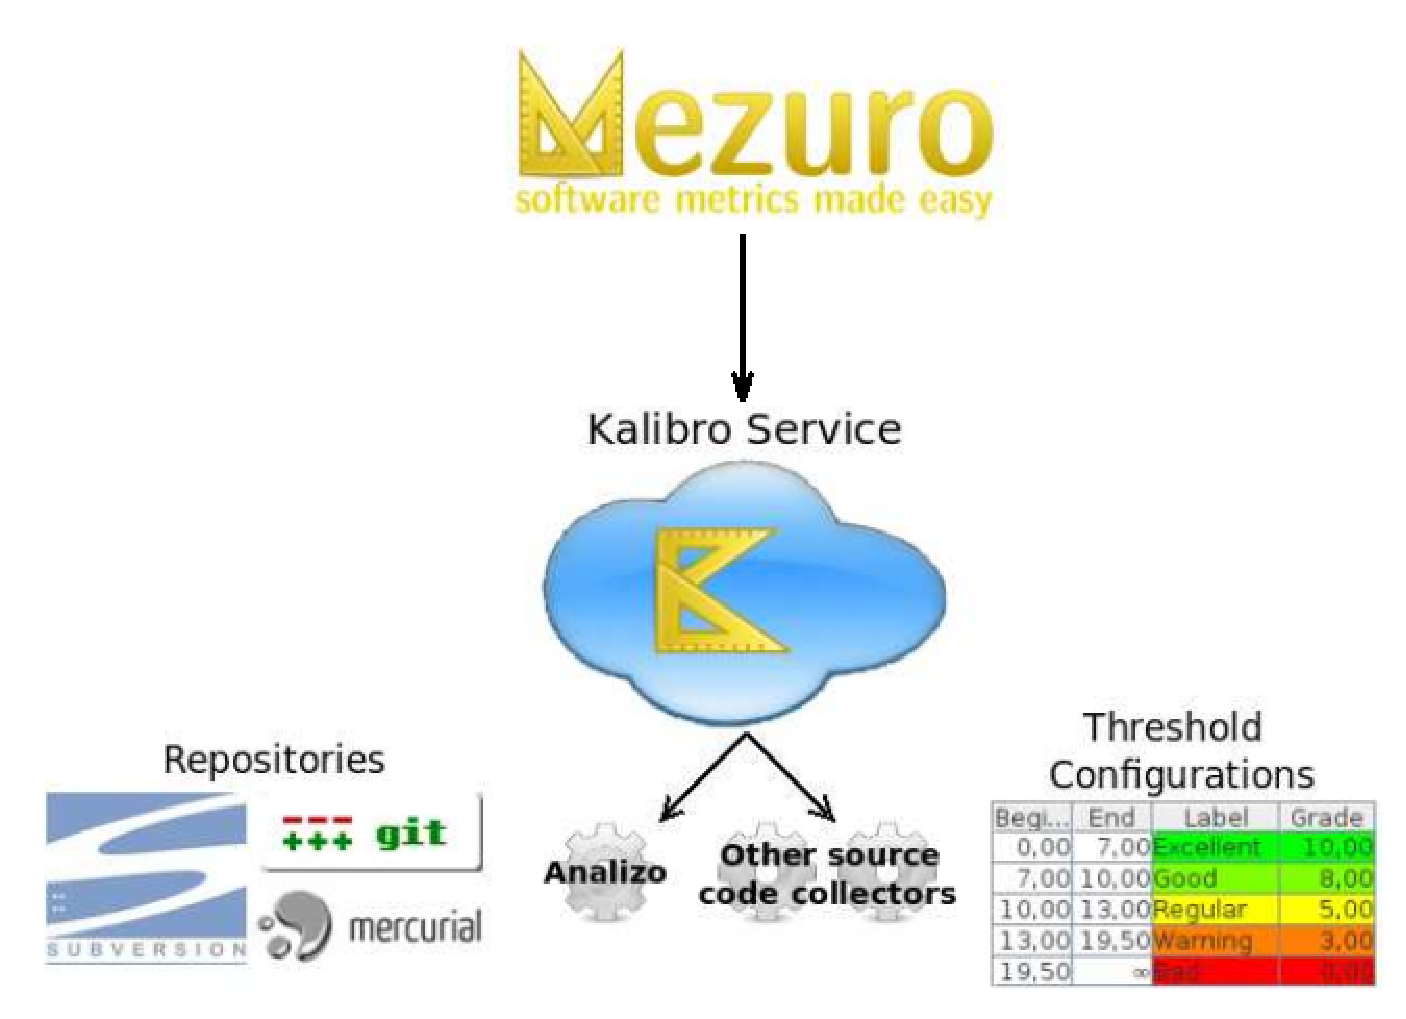
\includegraphics[width=0.6\textwidth]{mezuro-standalone-design}
\caption{Design de alto-nível do Mezuro. Editado de \cite{meirelles2010mezuro}}
\label{mezuro-design}
\end{figure}

Sem as restrições impostas pelo desenvolvimento do Noosfero, uma importante decisão arquitetural tomada pela equipe do Mezuro foi o desenvolvimento de uma \textit{gem} (para Ruby, equivalente a uma \textit{Lib} do Java) do Kalibro Metrics. Anteriormente, quando o Mezuro estava incorporado ao Noosfero, toda a interface de utilização do serviço do Kalibro estava implementada no próprio Mezuro. Com o desenvolvimento dessa \textit{gem}, esse serviço se torna mais reutilizável, resultando numa contribuição a toda a comunidade do Rails, já que em projetos desenvolvidos com esse arcabouço e necessitam utilizar serviços do Kalibro, bastam instalar e utilizar a \textit{gem}, sem a necessidade de reimplementar a interface do serviço.

\graphicspath{{figuras/}}
\begin{figure}[h]
\centering
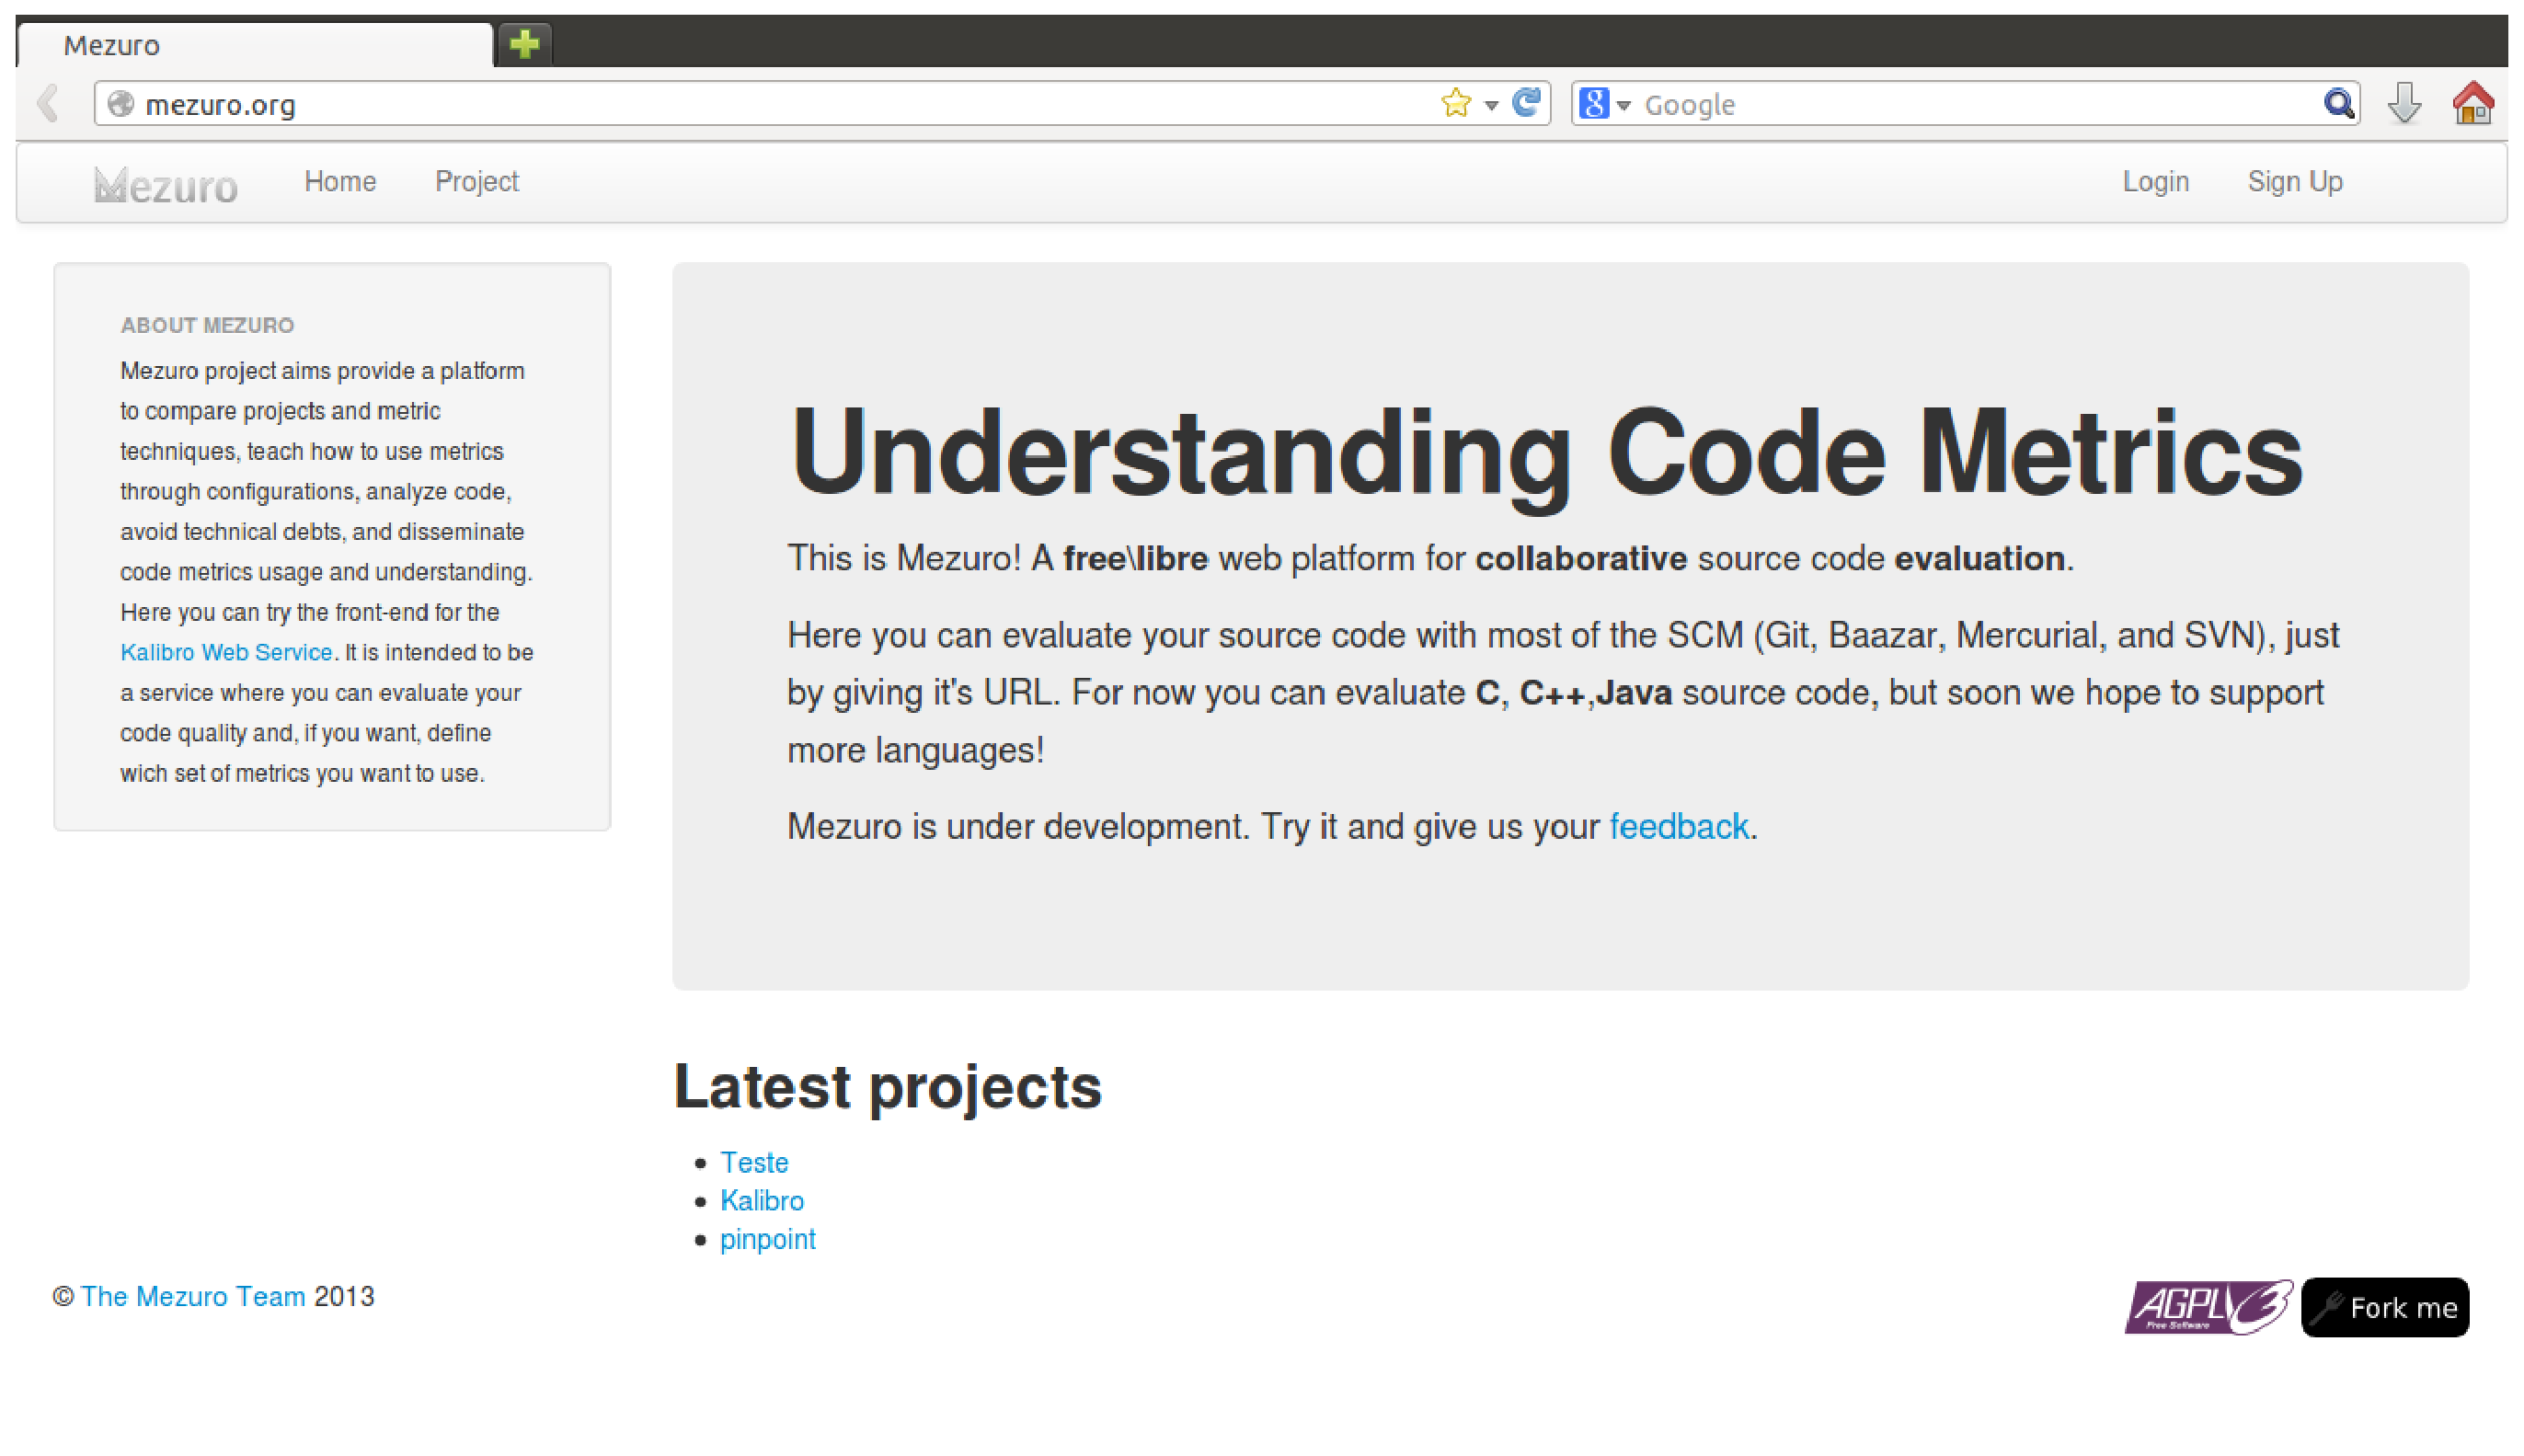
\includegraphics[width=0.7\textwidth]{mezuro-standalone}
\caption{Tela principal do Mezuro. Disponível em \url{http://mezuro.org/}}
\label{mezuro}
\end{figure}

Dentro da evolução do Mezuro, nesta primeira fase trabalho, como uma forma de conhecer a tecnologia e aprender a colaborar com o Mezuro, desenvolvemos a funcionalidade de inserção de repositórios nos projetos cadastrados para serem monitorados no Mezuro. De acordo com o diagrama da Figura \ref{class-diagram} é observado que um projeto possui diversos repositórios, os quais podem ser adicionados e removidos de um projeto, além de editados e visualizados. No caso da visualização é feito um processamento para que o usuário análise as métricas extraídas do código presente nesse repositório. 
%
Essa funcionalidade, desenvolvida ao decorrer deste trabalho, se encontra atualmente disponível na primeira versão do Mezuro como plataforma independente, lançada no mês de novembro de 2013,  ilustrada na Figura \ref{mezuro}.

\graphicspath{{figuras/}}
\begin{figure}[h]
\centering
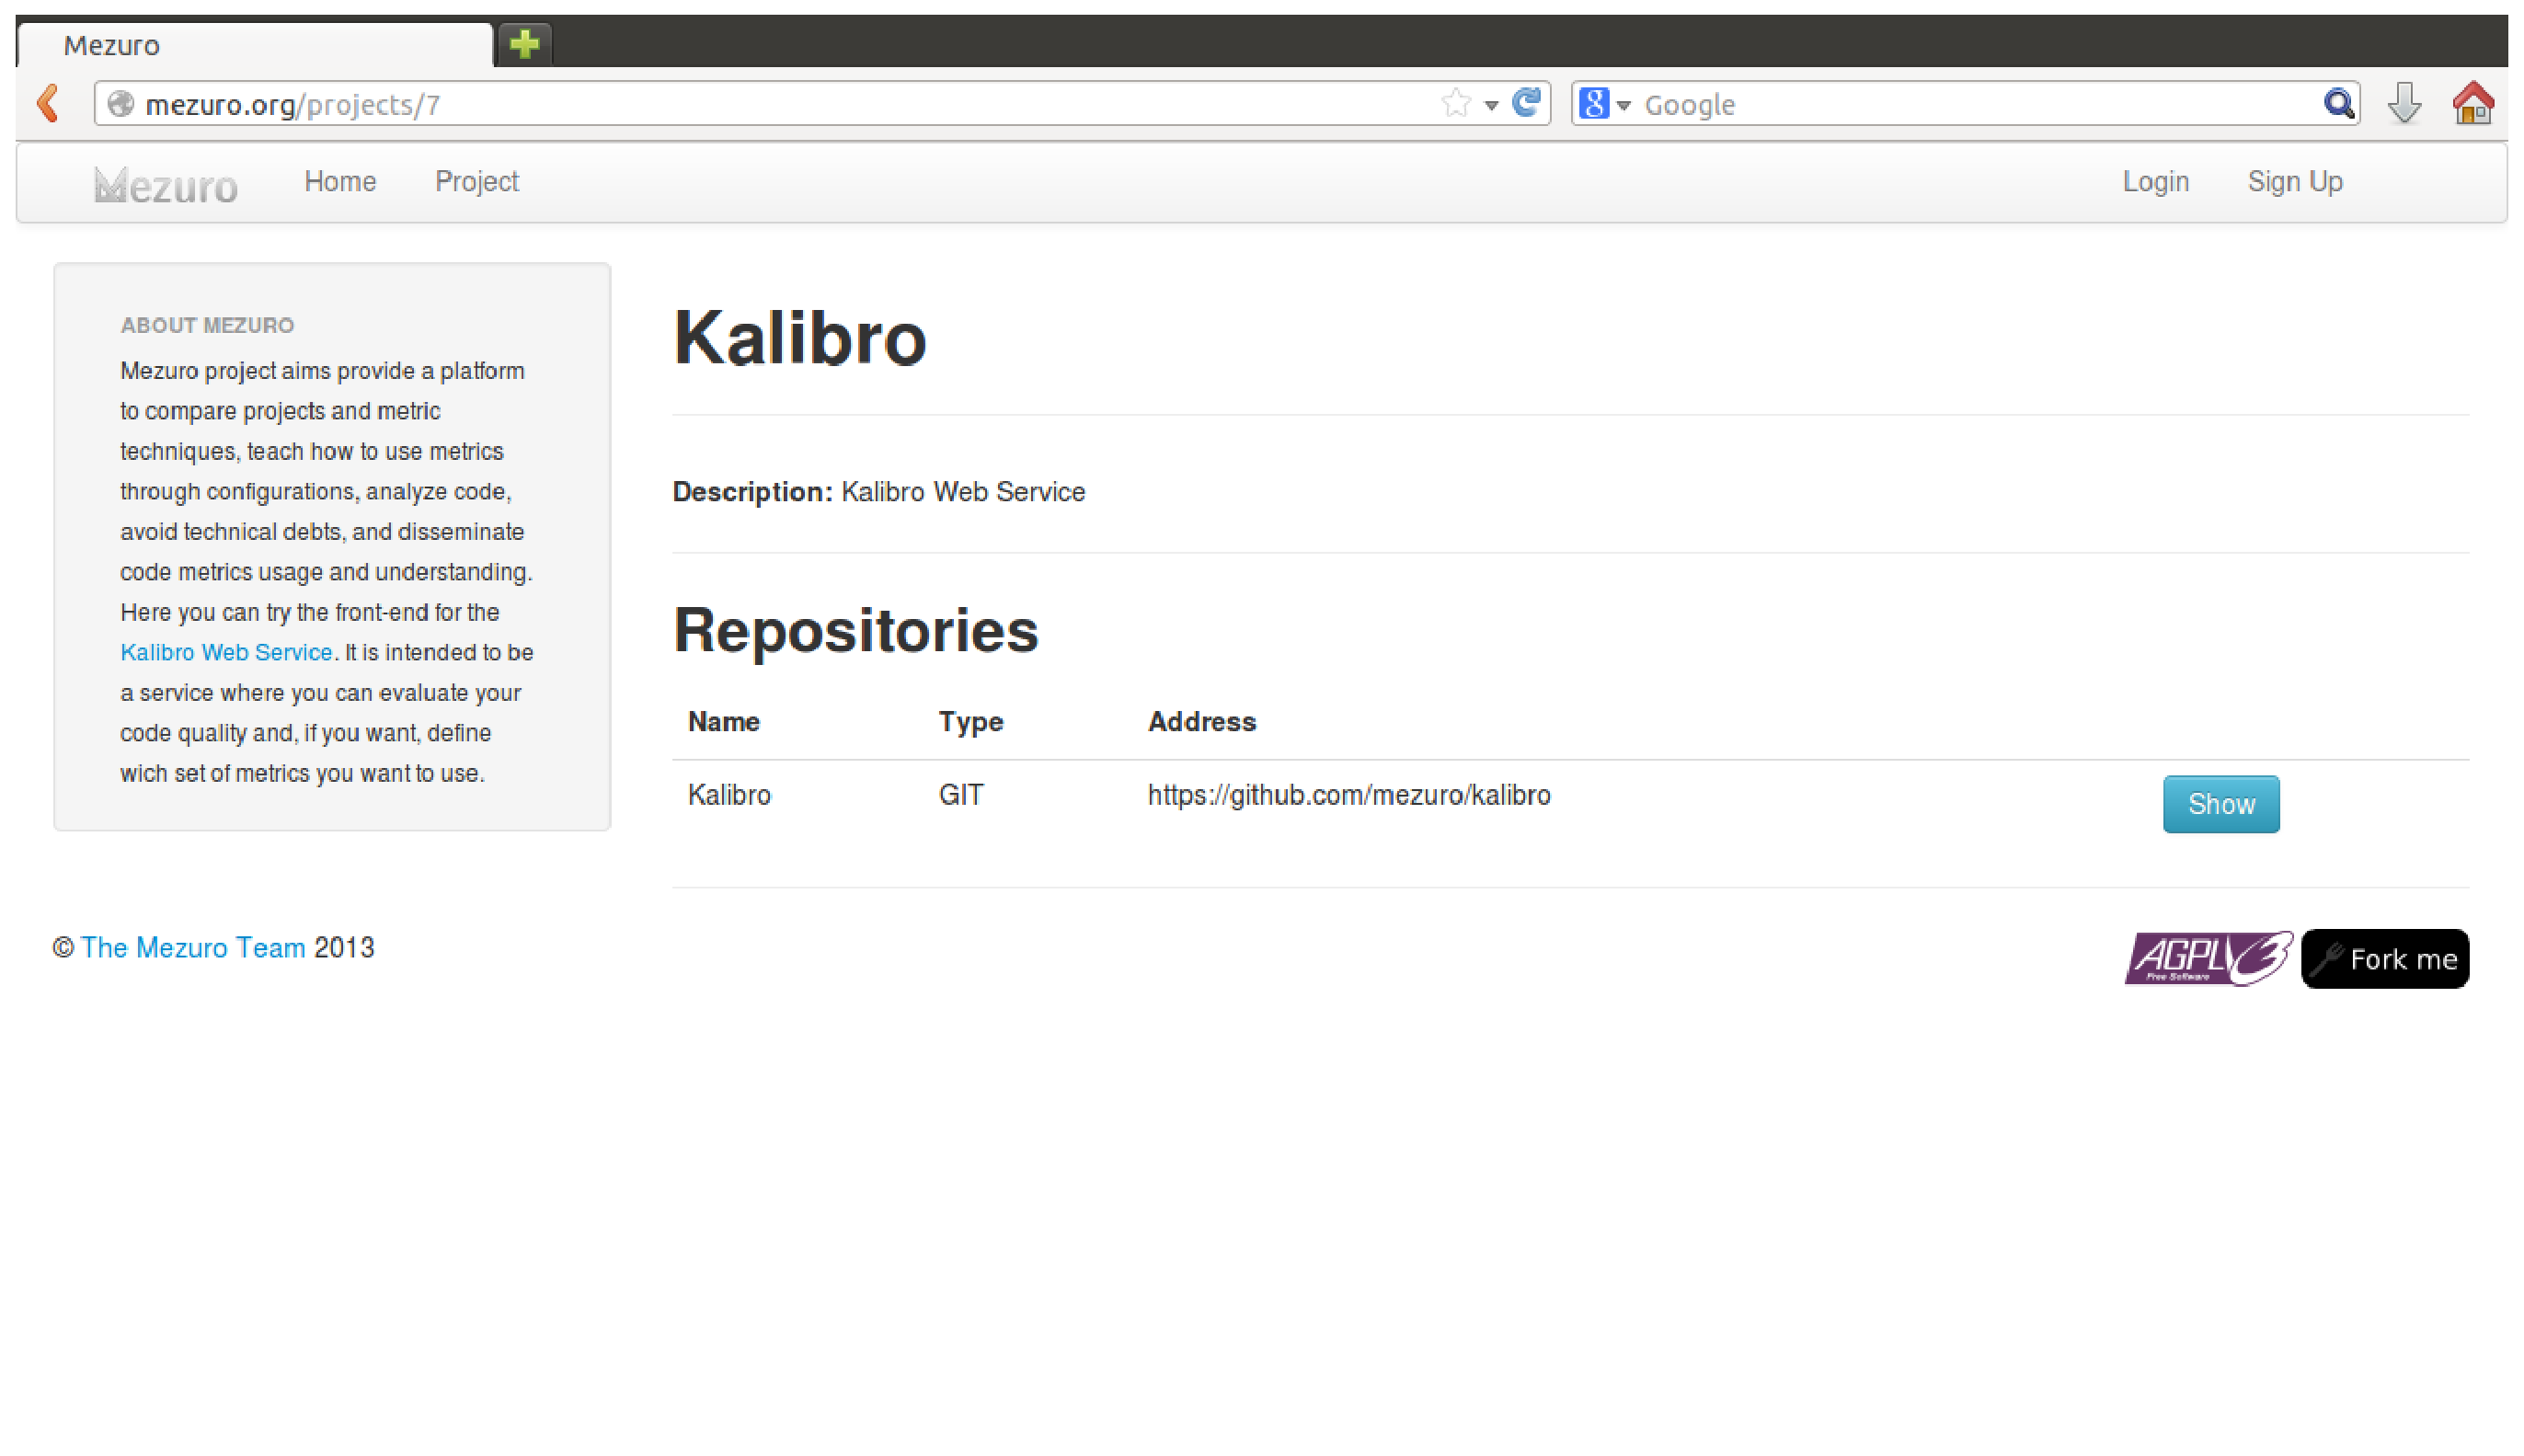
\includegraphics[width=0.7\textwidth]{mezuro-repositories}
\caption{Tela de visualização de um projeto}
\label{fig:mezuro-repositories}
\end{figure}

Ao clicar em algum projeto disponível no Mezuro, sua tela visualização é carregada. Nela são exibidas todos os repositórios realacionados a esse projeto. Na Figura \ref{fig:mezuro-repositories}, por exemplo, é exibida a tela do monitoramento do código do Kalibro cadastrado no Mezuro, assim como um único repositório associado a ele.

\graphicspath{{figuras/}}
\begin{figure}[h]
\centering
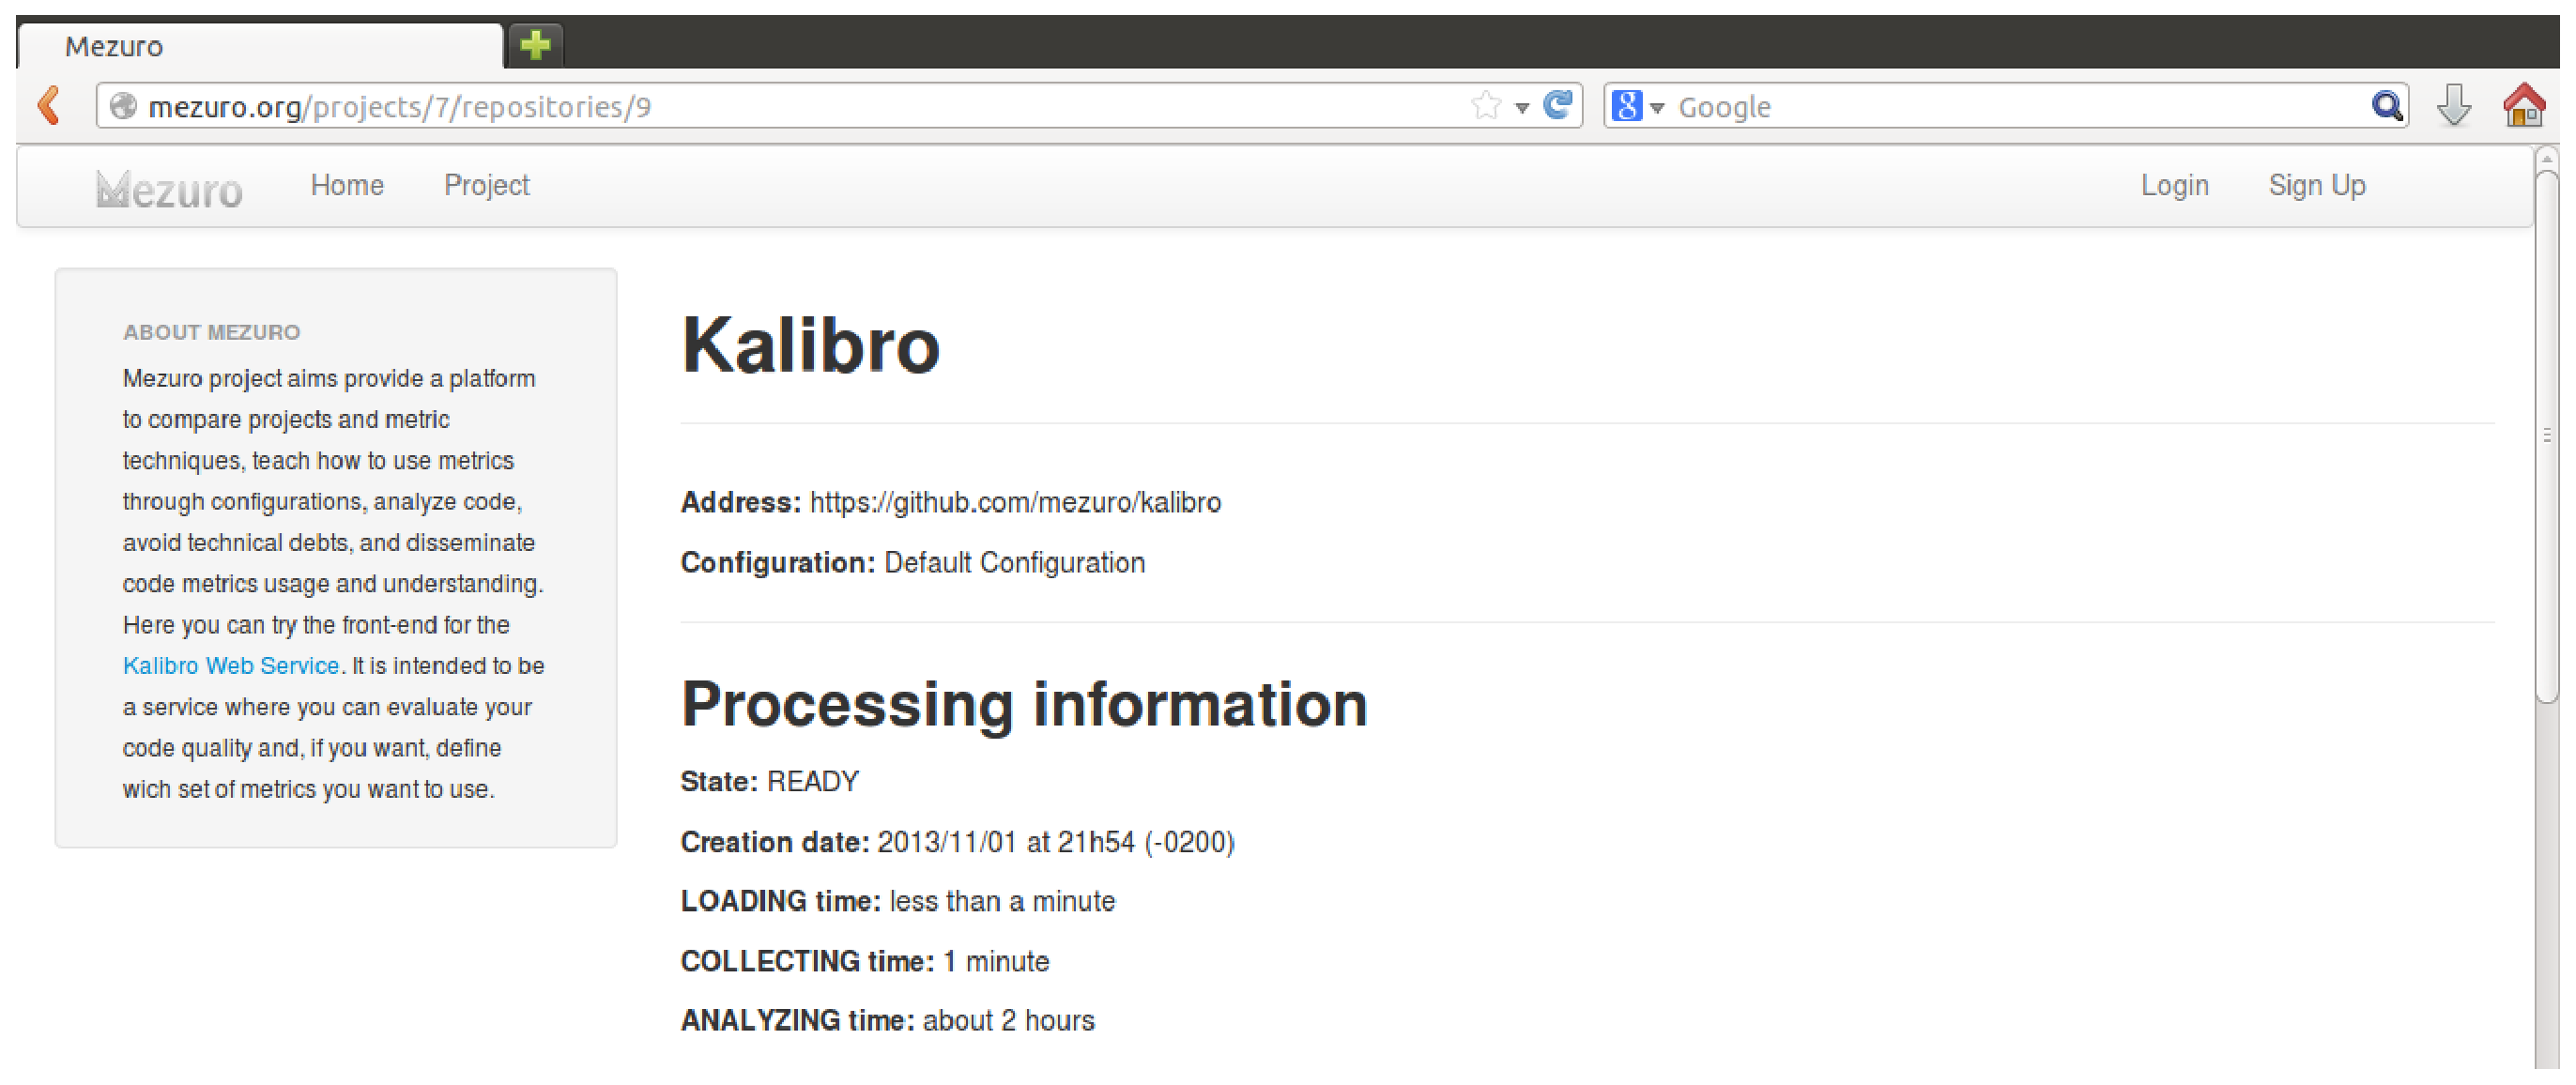
\includegraphics[width=0.7\textwidth]{mezuro-info}
\caption{Tela de informações do repositório}
\label{fig:mezuro-info}
\end{figure}

\graphicspath{{figuras/}}
\begin{figure}[h]
\centering
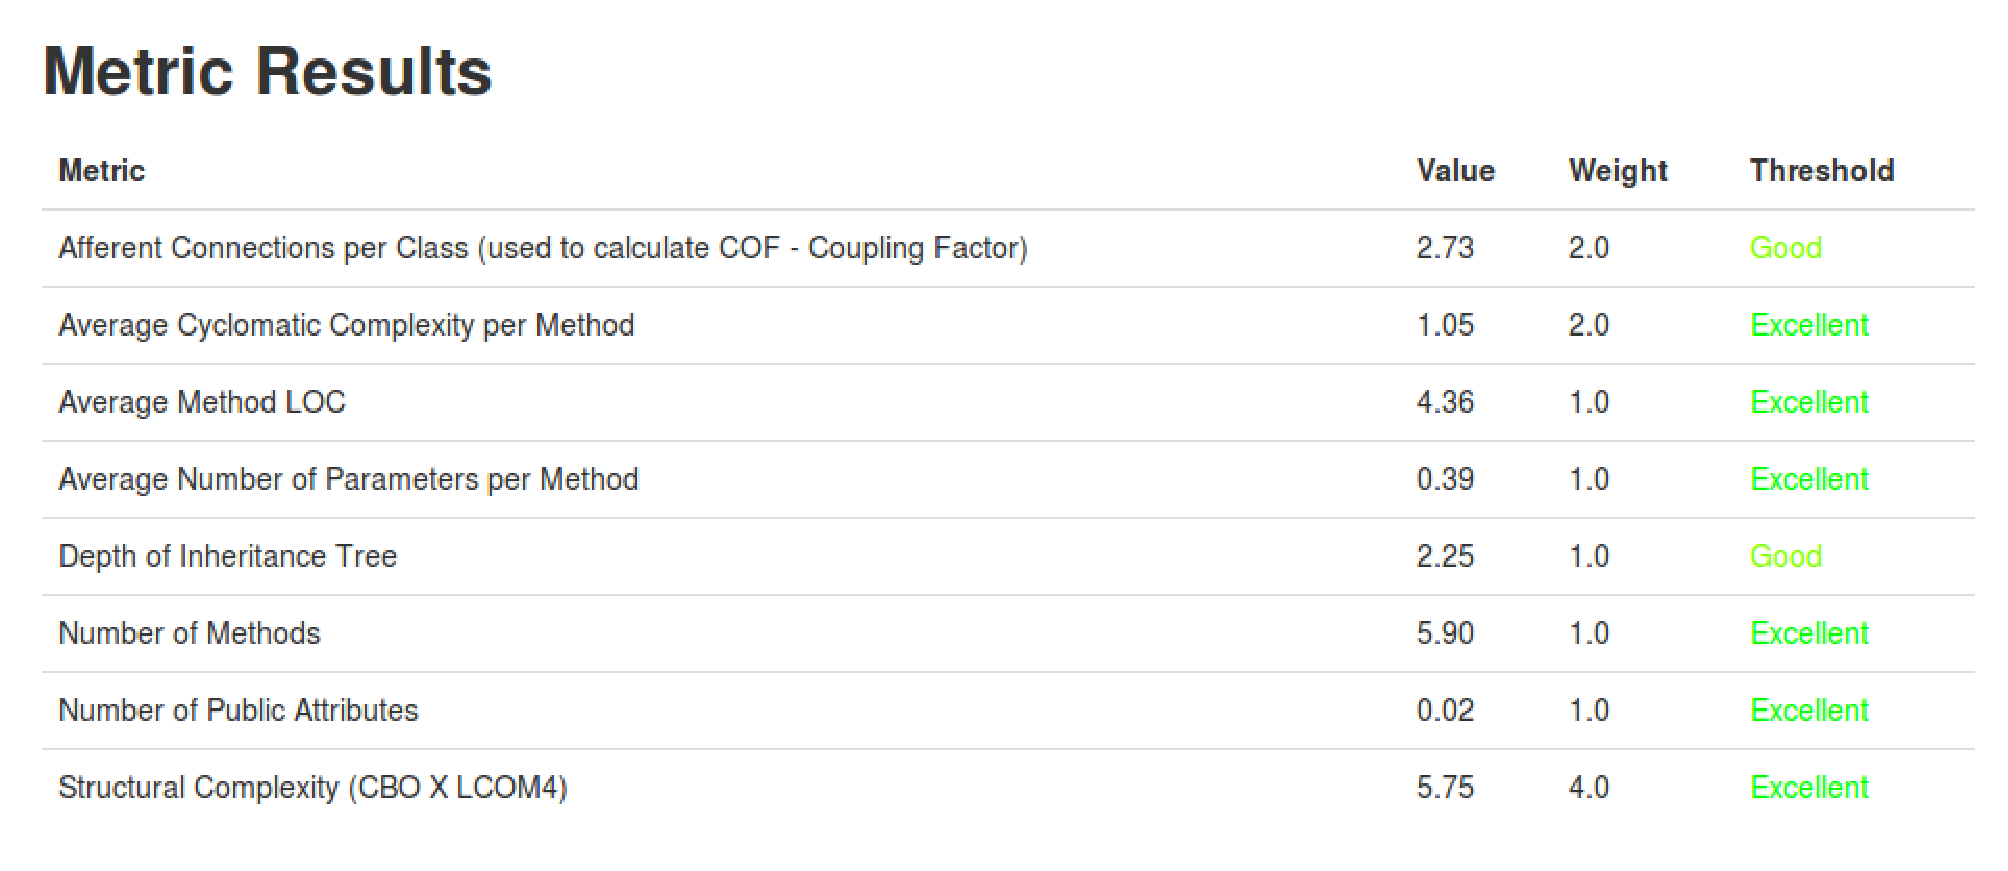
\includegraphics[width=0.7\textwidth]{mezuro-result}
\caption{Métricas do repositório após processamento}
\label{fig:mezuro-result}
\end{figure}

Ao clicar em visualizar um repositório, é feito um processamento desse, e a tela de detalhes do mesmo é carregada. A Figura \ref{fig:mezuro-info} e \ref{fig:mezuro-result} são os resultados do processamento do único repositório associado ao projeto Kalibro monitorado pelo Mezuro.
%
A Figura~\ref{fig:mezuro-info} exibe informações gerais do processamento do reposítório, como a configuração, estado, data de criação e tempo de processamento. A Figura~\ref{fig:mezuro-result} mostra o conjunto de métricas relacionas à configuração do repositório processado (uma configuração \textit{default}, por exemplo), assim como os intervalos e interpretação de cada uma dessas métricas.

\graphicspath{{figuras/}}
\begin{figure}[h]
\centering
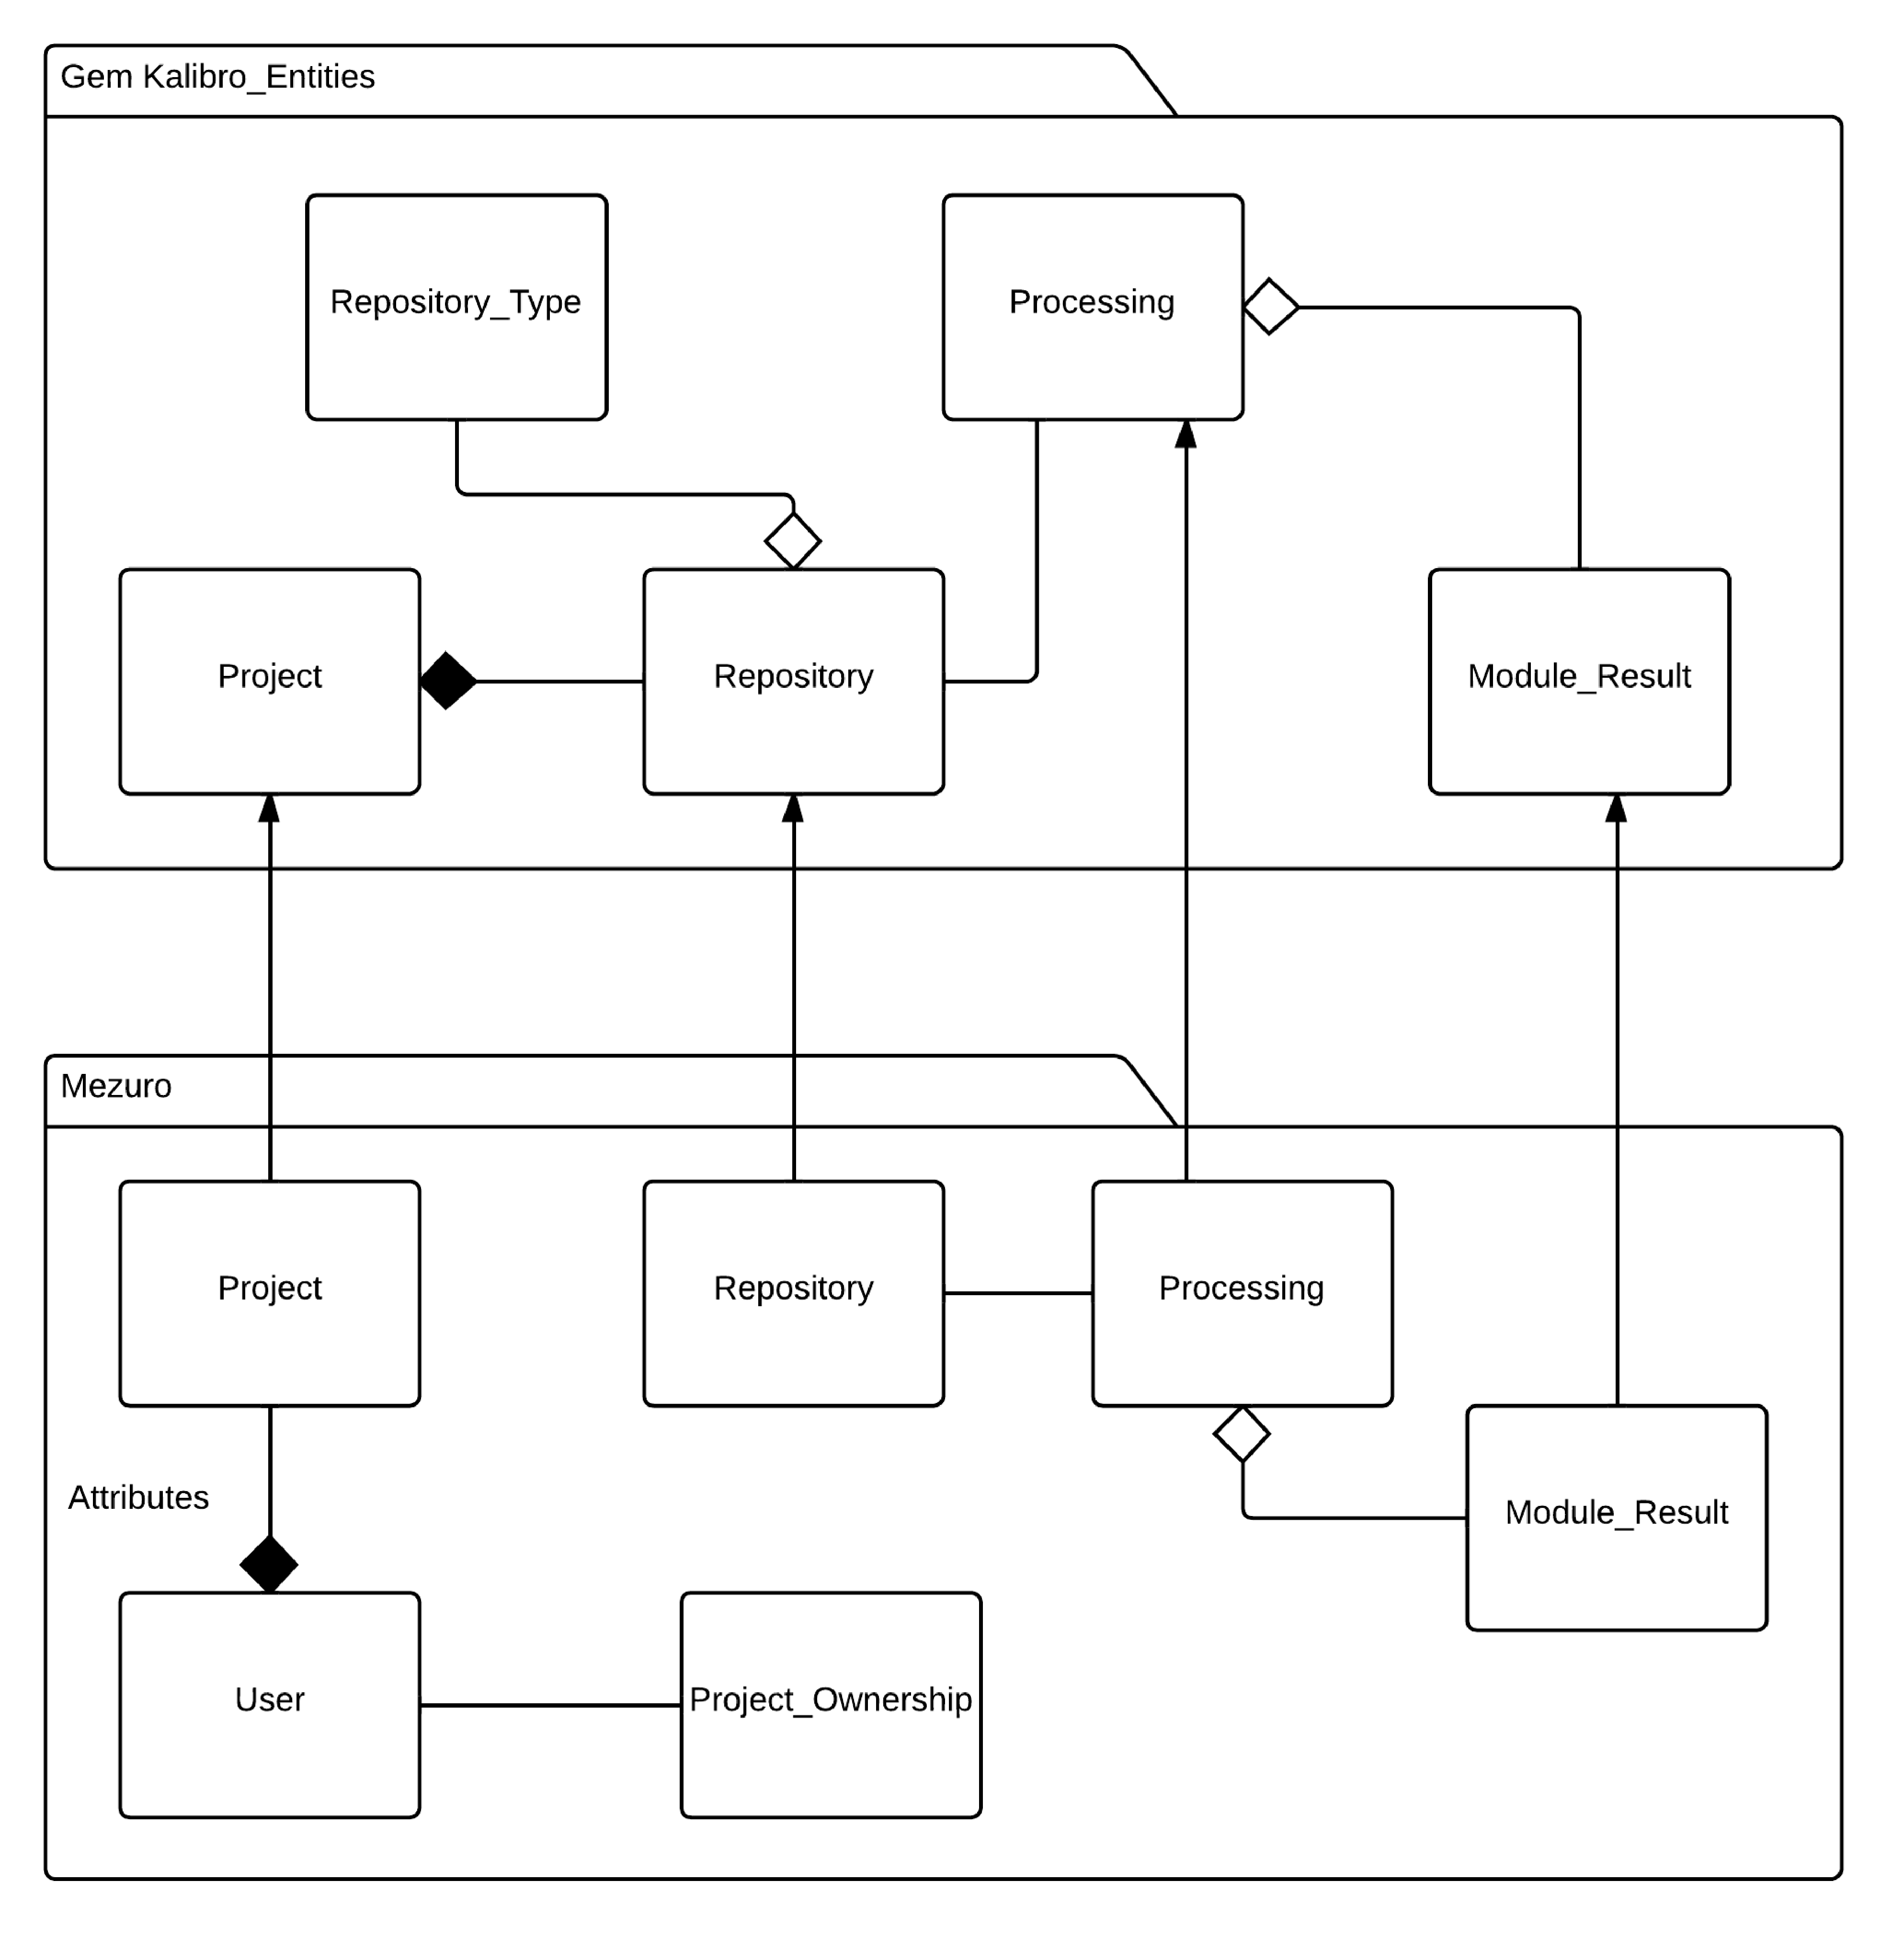
\includegraphics[width=0.6\textwidth]{class-diagram-mezuro}
\caption{Diagrama de classes simples do Mezuro}
\label{class-diagram}
\end{figure}

Por fim, a Figura \ref{class-diagram} apresenta um diagrama de classes que representa as entidades já implementadas no Mezuro como plataforma independente. A classe \textit{Project} representa o projeto a ser analisado. Um projeto pode conter vários repositórios, de onde as métricas são extraídas.  Um repositório pode ser de vários tipos, Git\footnote{\url{http://git-scm.com/}}, Subversion\footnote{\url{http://subversion.apache.org/}}, Bazaar\footnote{\url{http://bazaar.canonical.com/en/}} e Mercurial\footnote{\url{http://mercurial.selenic.com/}}. A classe \textit{Processing} representa o processamento de um repositório para obter os resultados das métricas extraídas de acordo com a configuração selecionada. E finalmente, a classe \textit{Module-Result} representa o resultado do processamento de um repositório. Uma configuração representa um conjunto de métricas, um intervalo para cada uma delas, além da interpretação de cada métrica após o processamento de um repositório. Terminar de  migrar todas essas funcionalidades, que já estavam implementadas no Mezuro Plugin, é o ponto em que está esse processo de evolução do Mezuro.

